%************************************************
\chapter{Thin Layer Chromatography (Constituent Detection)}
%************************************************
\begin{flushright}
January 21, 2013
\end{flushright}
\section{Aim}
To find the constituents of the mixture samples given, which contain two of the following each: 
\begin{enumerate}[A)]
	\item Resorcinol
	\item p-Hydroxybenzaldehyde
	\item 2,4 - Dinitrophenylhydrazine
	\item p-Nitro Aniline
\end{enumerate}
and to find the corresponding $R_f$ values, using suitable solvent systems.

\section {Chemicals Required}
	\begin{enumerate}
		\item Resorcinol
		\item p-Hydroxybenzaldehyde
		\item 2,4 - Dinitrophenylhydrazine
		\item p-Nitro Aniline
	\end{enumerate}

\section{Theory}
	The theory here is rather straight forward. We already know that the sample contains two components. We, on a TLC, make three spots, the extreme right comprising of only, say A, the middle comprising of A and the mixture, and the extreme left spot, comprising of only the mixture. Now as shown in the diagram, we'll obtain three spots in the middle (called the co-spot), if A is not already present in the compound. If A is present, then only two spots will appear in the middle.\par
	It is the same as saying that the extreme left should have fewer spots than the co-spot if A is not present, in general, and the `extra spot' in the co-spot, must match with the spot of A on the extreme right.

	\begin{figure}[bth]
		\begin{center}
			
\includegraphics[width=0.8\linewidth]{gfx/e2_separate}
		\end{center}
	\caption[Diagrammatic representation of the test setup]{\label{1A_slides}}
	\end{figure}


\section{Procedure}	
	\begin{enumerate}
		\item Preparing the TLC plates (same as the previous experiment, repeated here for convenience)
		\begin{enumerate}
			\item Prepared a silica slurry, using silica and ethyl acetate
			\item Dipped two glass slides, held together, into the solution, to coat about eighty percent of it with the slurry.
			\item Allowed them to dry (could blow air on it to accelerate the process) and them separated them.	
		\end{enumerate}
		\item Visibility Chamber (again, same)
		\begin{enumerate}
			\item Added a few granules of Iodine with silica granules dominant in number, in a beaker, covered with a watch glass.
		\end{enumerate}
		\item Various concentrations ($5\%$, $10\%$ and $20\%$) Ethyl Acetate Soln. in Hexane
		\begin{enumerate}
			\item Using a measuring cylinder, measured the required volume of Ethyl Acetate and the made the volume 10 mL using Hexane. Transferred the contents in a suitable beaker and covered it with a watch glass.
		\end{enumerate}
		\item Diluted the given solutions of A, B, C, D, Mixture 1 and Mixture 2 appropriately and using a capillary tube, put the spots as described in the theory, using compounds A, B, C and D, one after the other, on the TLC plate, near the silica coated edge. Also, marked physically, by a method suitable, the position of the spot. \marginpar {\Maggie Our dilutions were not sufficient the first time we attempted this and we had to redo the entire procedure}
		\item Placed the TLC place, carefully (it's fragile) inside the Ethyl Acetate Soln. (its concentration was changed progressively in accordance with displacement of the spots), such that the spot is above the level of the solution initially and covered it again, with the watch glass. \marginpar {\Maggie We once ended up dipping the spots in the solution itself, which lead to trouble later}
		\item Kept a watch on the TLC and removed it as soon as the solvent crossed about $90\%$ of the height of the silica coating and placed it cautiously in the Visibility Chamber, until the spots became visible. This is the same as before, except that we setup two chambers simultaneously to speeden up the process.
		\item Now marked the positions of all the spots, deduced presence of the substance taken and also calculated the $R_f$ value for A, B, C and D.
	\end{enumerate}
\section{Observations and Results}
	Mixture 1 was found to be constituted of compounds A and B, viz. Resorcinol and p-Hydroxybenzaldehyde. In a $20\%$ system, we observed:
	\begin{enumerate}
		\item Resorcinol : $R_f=0.129$
		\item p-Hydroxybenzaldehyde : $R_f=0.477$
		\item 2,4 - Dinitrophenylhydrazine : $R_f=0.028$
		\item p-Nitro Aniline : $R_f=0.202$
	\end{enumerate}

	Mixture 2 was found to be constituted of compounds C and D, viz. 2,4-Dinitrophenylhydrazine and p-Nitro Aniline. In a $20\%$ system, we observed:
	\begin{enumerate}
		\item Resorcinol : $R_f=0.129$
		\item p-Hydroxybenzaldehyde : $R_f=0.422$
		\item 2,4 - Dinitrophenylhydrazine : $R_f=0.085$
		\item p-Nitro Aniline : $R_f=0.259$
	\end{enumerate}
	
	For details, please refer to \autoref{2_mix1} and \autoref{2_mix2}

	\begin{figure}[bth]
		\begin{center}
			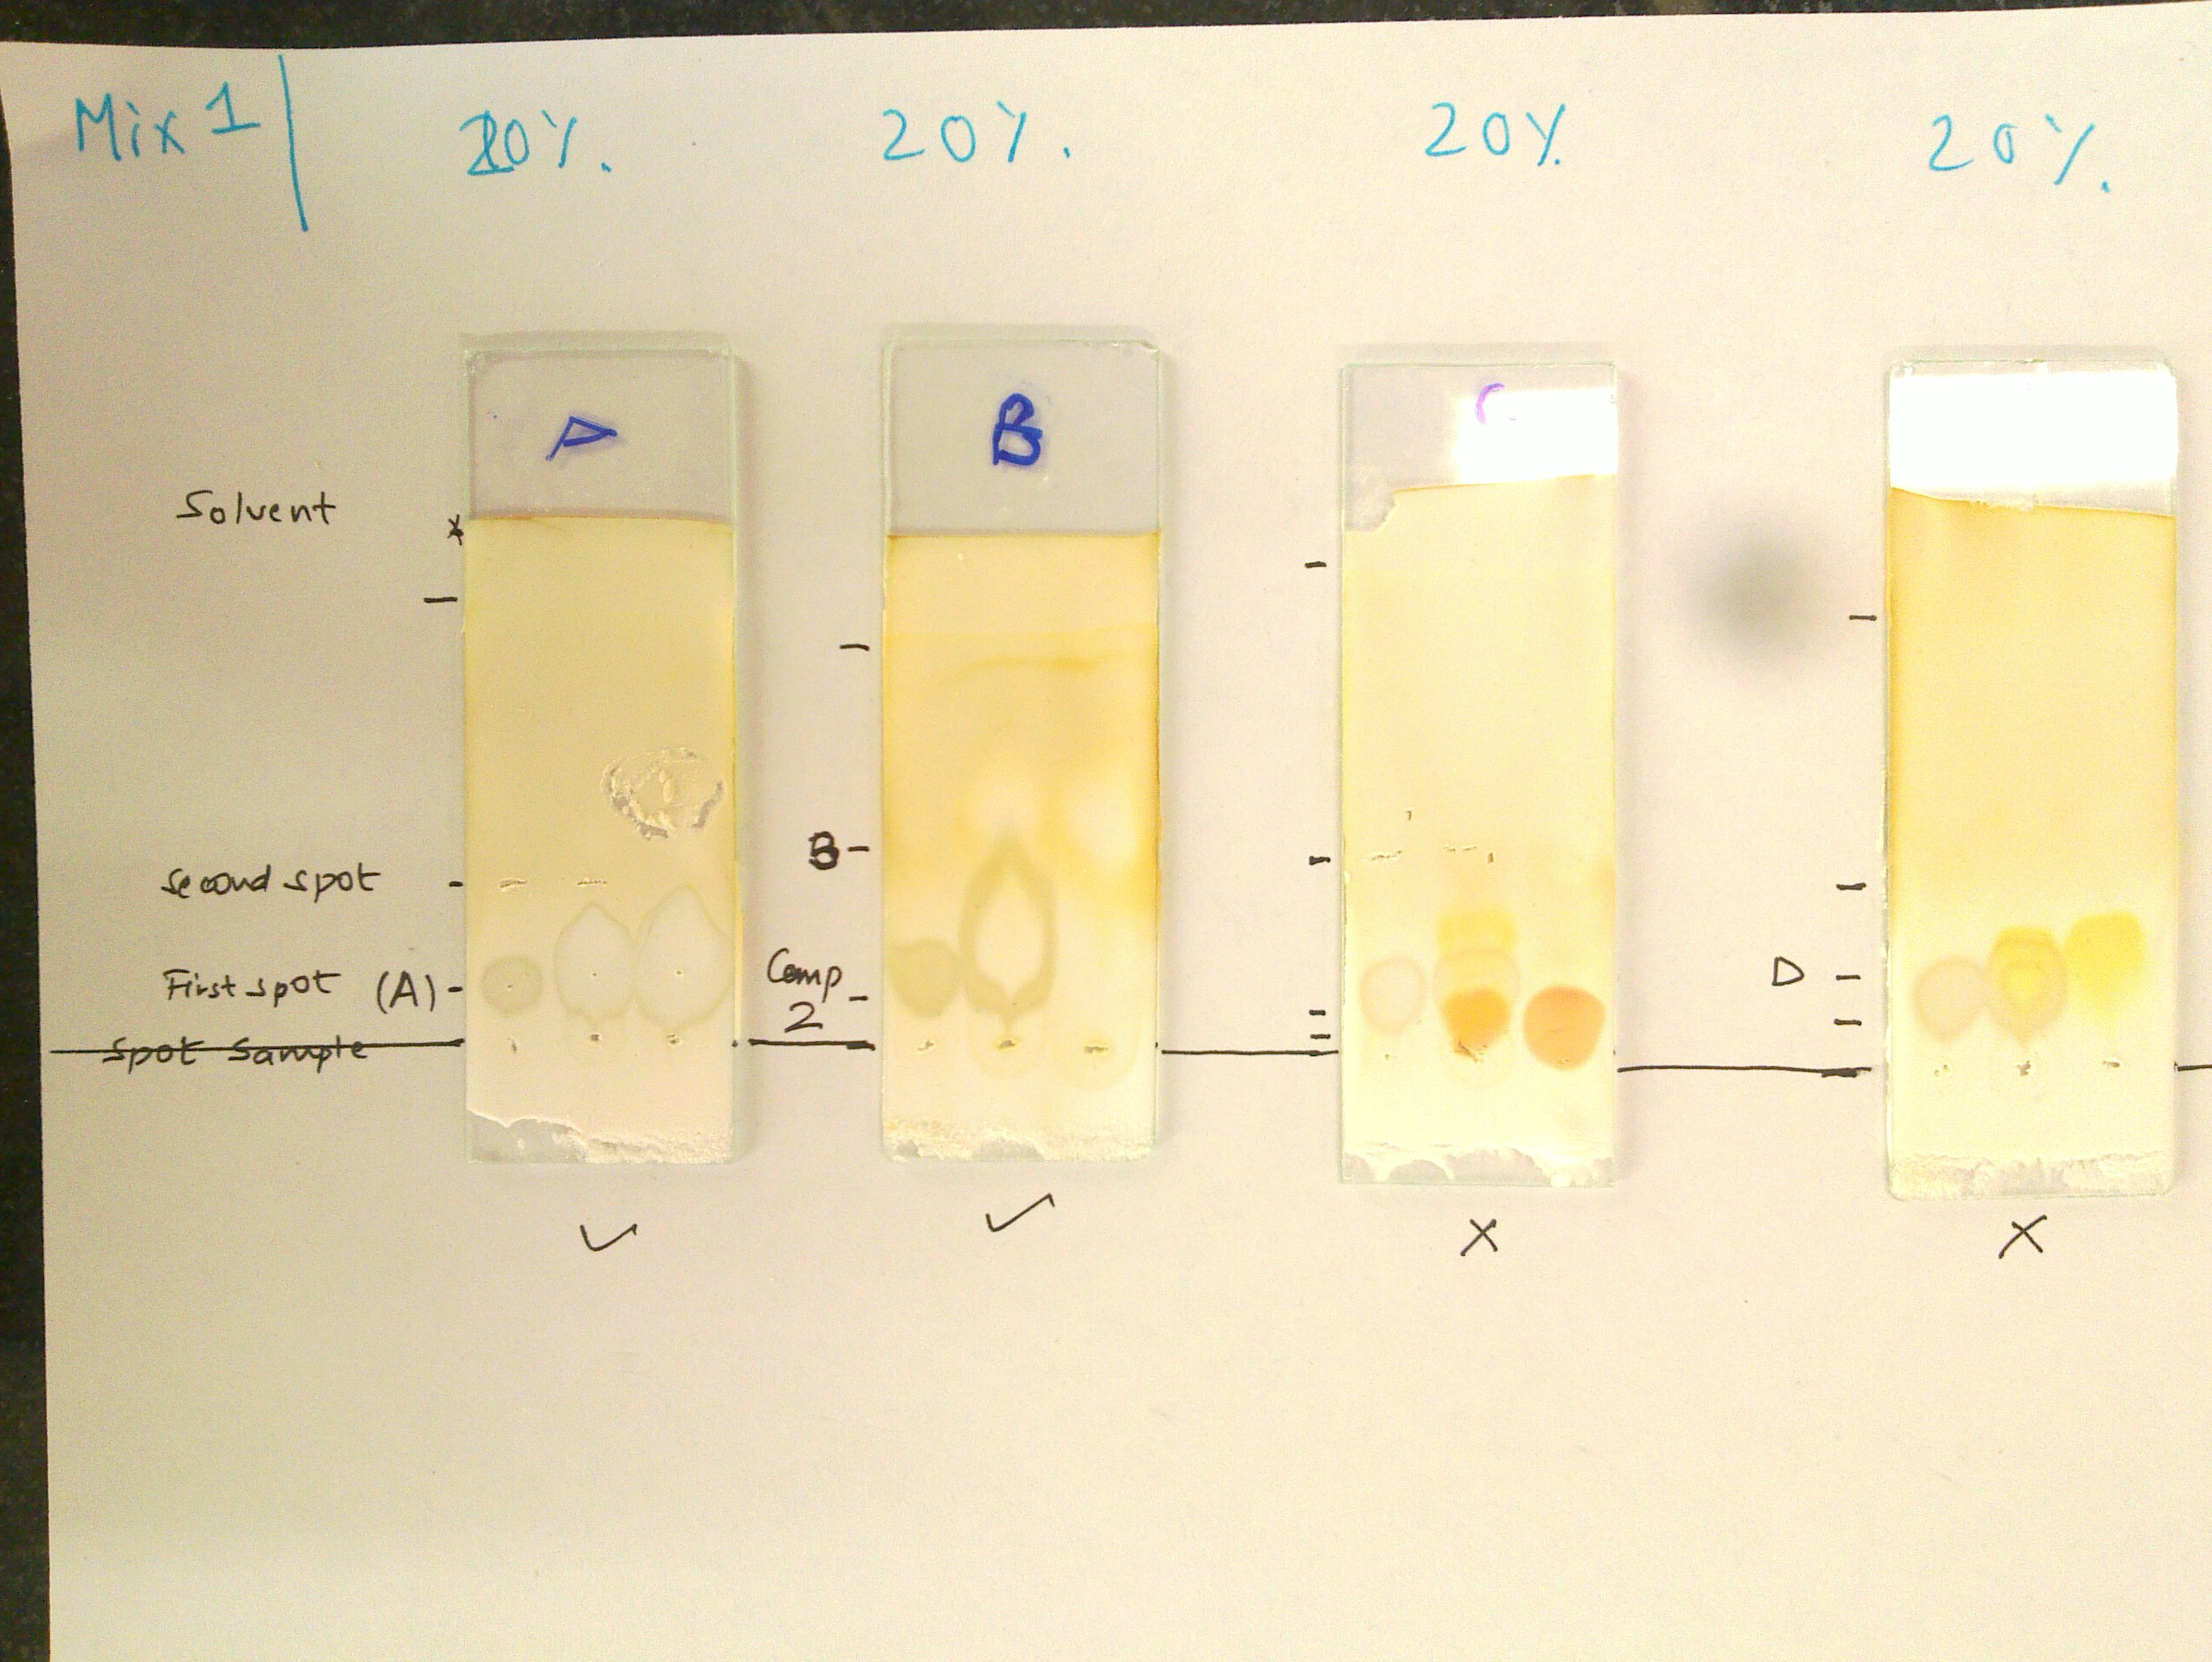
\includegraphics[width=1.2\linewidth]{gfx/e2_mix1}
		\end{center}
	\caption[TLC plates for Mixture 1]{\label{2_mix1}}
	\end{figure}
	\begin{figure}[bth]
		\begin{center}
			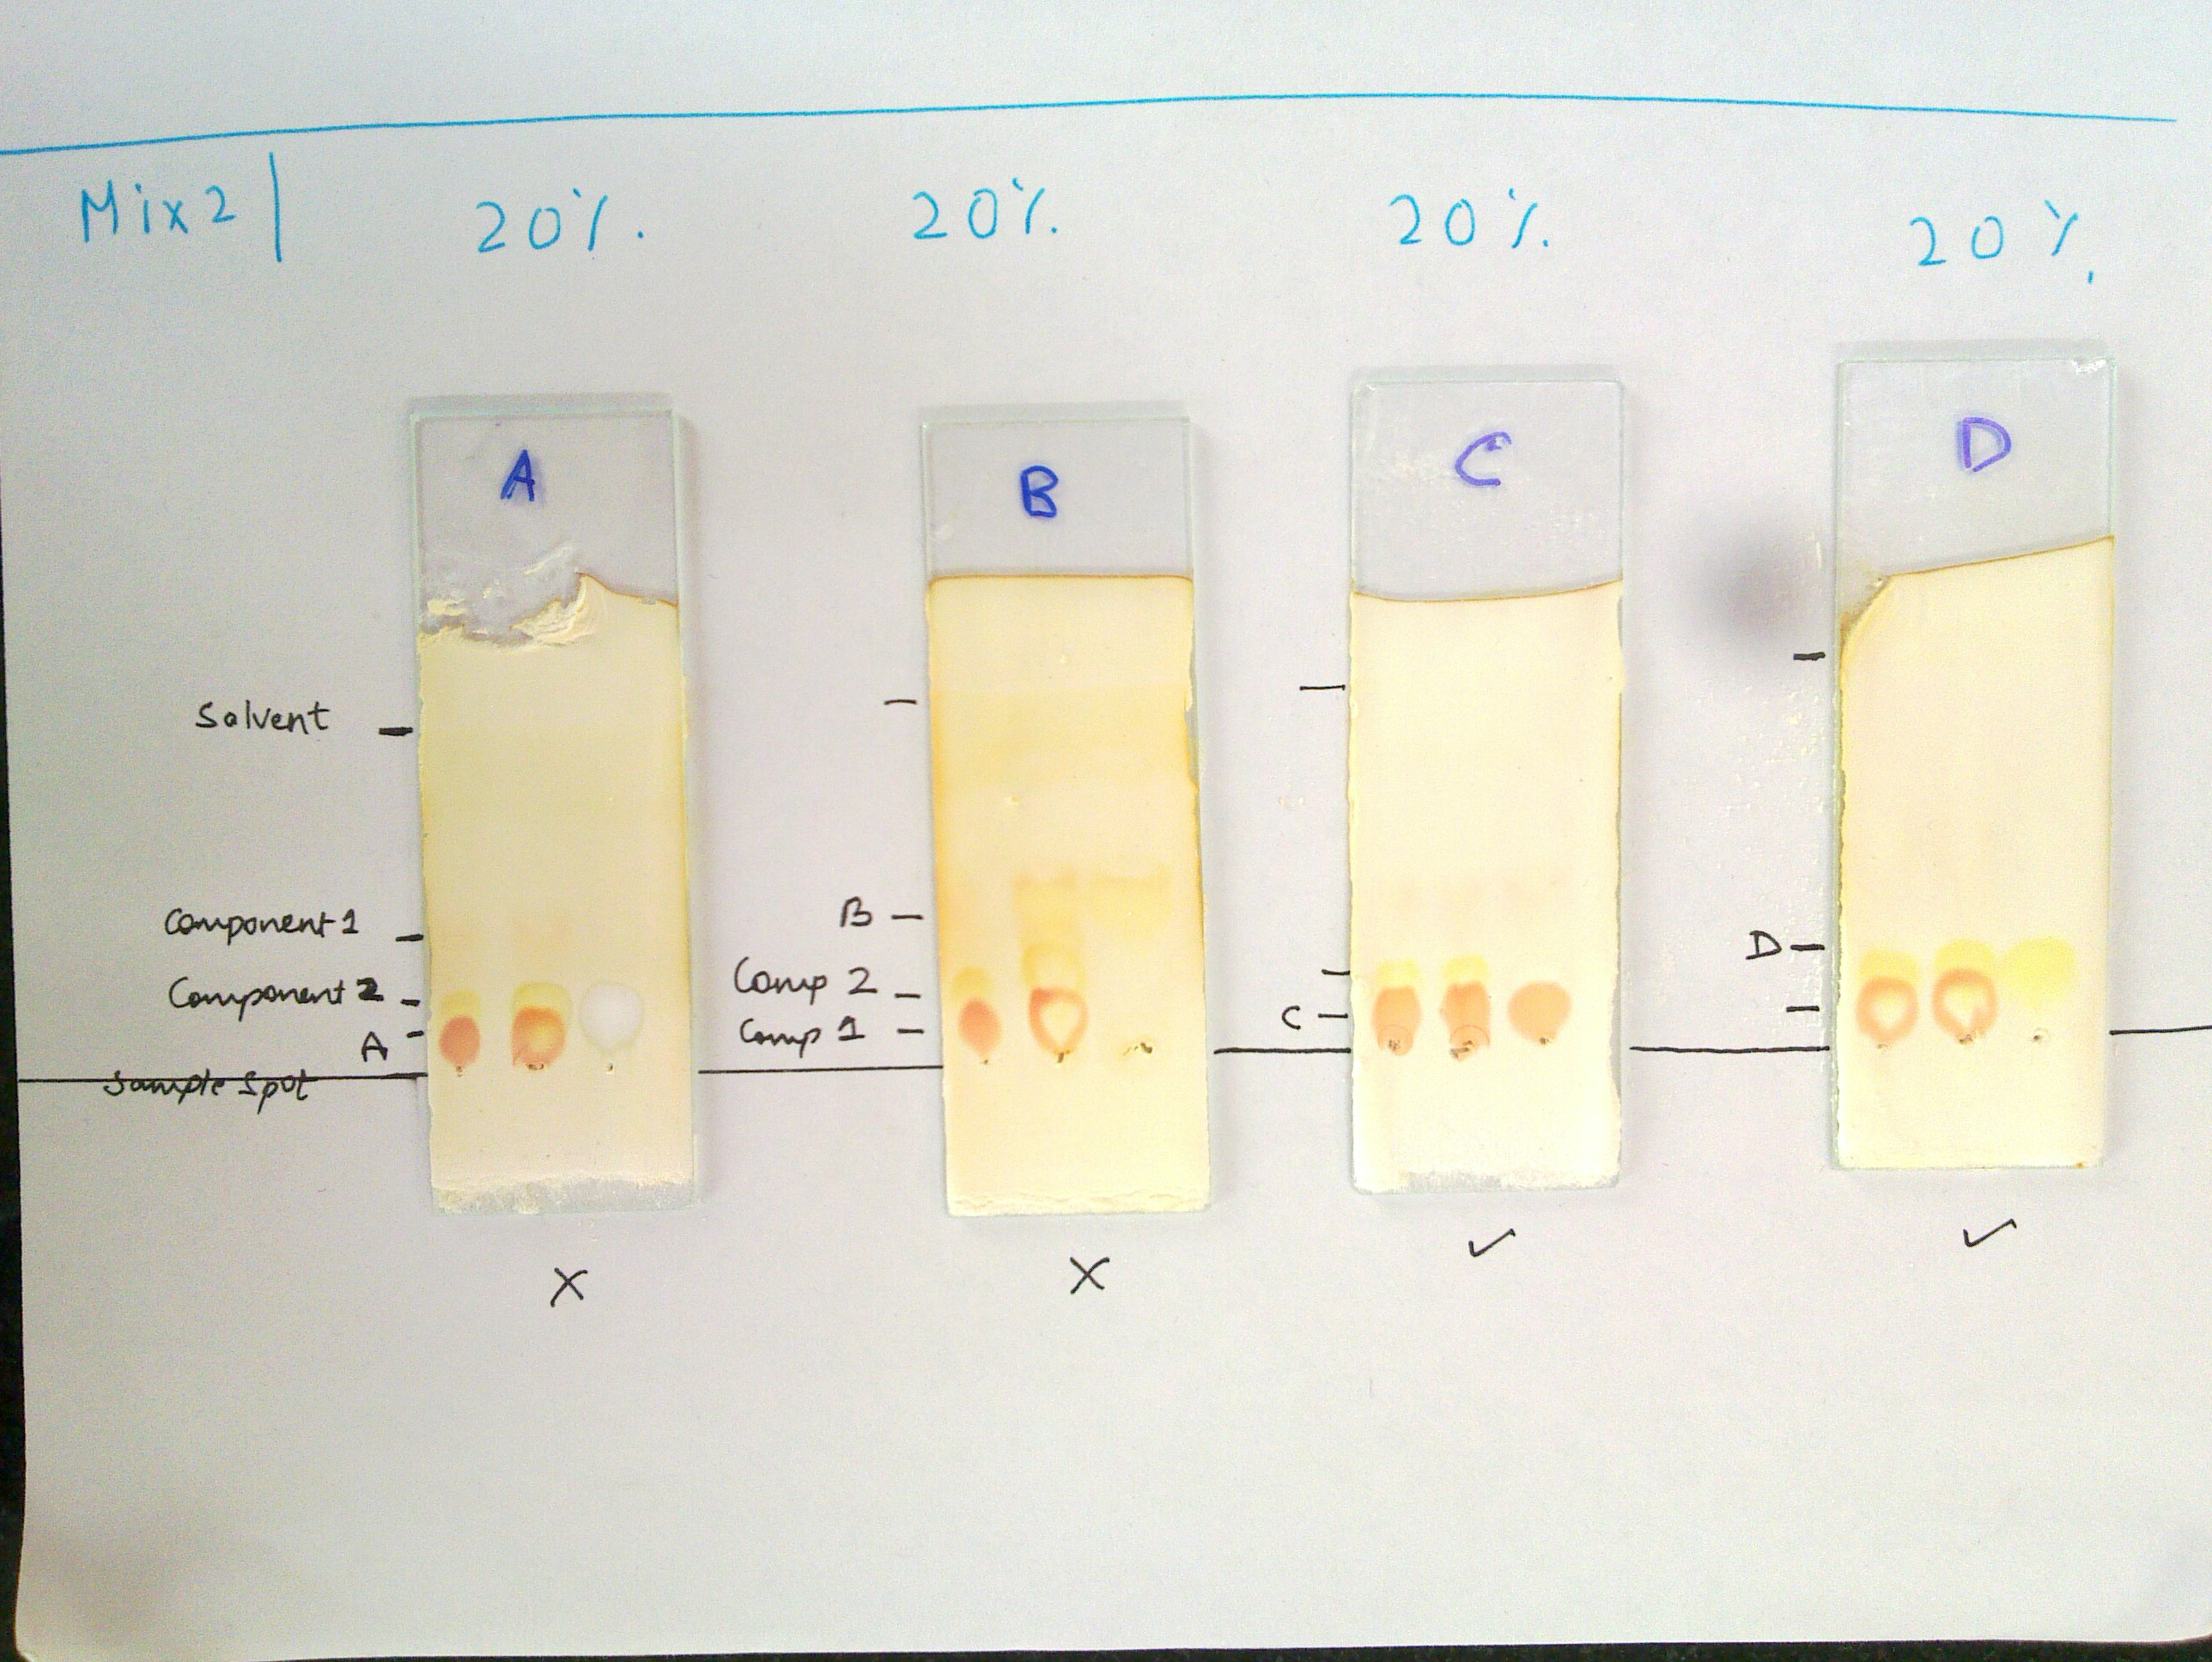
\includegraphics[width=1.2\linewidth]{gfx/e2_mix2}
		\end{center}
	\caption[TLC plates for Mixture 2]{\label{2_mix2}}
	\end{figure}

\section{Precaution}
	Precautions are same as those in the previous experiment, viz.
	\begin{enumerate}
		\item The slurry shouldn't be very thick
		\item Cover the beakers with a watch glass to ensure there's no loss of volatile substances (minimal that is)
		\item The coating is very fragile, thus the TLC plates must be handled with caution
	\end{enumerate}	
\section{Acknowledgements}
I thank Dr. R Vijaya Anand for his guidance during the experiment. I also acknowledge the contribution of my lab partners, Prashansa and Srijit for performance of the same. I especially thank them for maintaining their calm while we were forced to repeat the experiment numerous times.